\documentclass[preview,border=7pt]{standalone}
\usepackage{amsmath,amssymb,xcolor}
\usepackage{tikz}
\usetikzlibrary{arrows.meta}
\definecolor{acc}{RGB}{47,143,132}
\definecolor{cyn}{RGB}{6,182,212}
\definecolor{amb}{RGB}{245,158,11}
\begin{document}
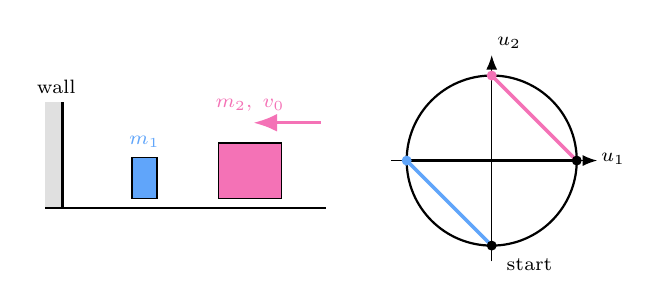
\begin{tikzpicture}
\definecolor{blu}{RGB}{96,165,250}
\definecolor{pnk}{RGB}{244,114,182}
%% --- lab (blocks placed from sim resetState, uniformly scaled) ---
\fill[black!12] (-0.22,-0.12) rectangle (0.0,1.22);
\draw[line width=1.15pt] (0,-0.12) -- (0,1.22);
\node at (-0.08,1.42) {\scriptsize wall};
\draw[line width=.9pt] (-0.22,-0.12) -- (3.35,-0.12);
\fill[blu] (0.88,0.0) rectangle (1.20,0.52);
\draw[line width=.6pt] (0.88,0.0) rectangle (1.20,0.52);
\fill[pnk] (1.98,0.0) rectangle (2.78,0.70);
\draw[line width=.6pt] (1.98,0.0) rectangle (2.78,0.70);
\draw[-{Latex}, pnk, line width=1.25pt] (3.28,0.96) -- (2.42,0.96);
\node[blu] at (1.04,0.72) {\scriptsize $m_1$};
\node[pnk] at (2.38,1.18) {\scriptsize $m_2,\;v_0$};
%% --- energy circle: N=0 states (0,-1) -> (-1,0) -> (1,0) -> (0,1) ---
\begin{scope}[shift={(5.45,0.48)}]
\draw[line width=.8pt] (0,0) circle (1.08);
\draw[line width=.35pt] (-1.28,0) -- (1.28,0);
\draw[line width=.35pt] (0,-1.28) -- (0,1.28);
\draw[-{Latex}, line width=.5pt] (1.08,0) -- (1.34,0);
\draw[-{Latex}, line width=.5pt] (0,1.08) -- (0,1.34);
\node at (1.54,0.02) {\scriptsize $u_1$};
\node at (0.22,1.50) {\scriptsize $u_2$};
\draw[blu, line width=1.25pt] (0,-1.08) -- (-1.08,0);
\draw[line width=1.25pt] (-1.08,0) -- (1.08,0);
\draw[pnk, line width=1.25pt] (1.08,0) -- (0,1.08);
\fill (0,-1.08) circle (1.8pt);
\fill[blu] (-1.08,0) circle (1.8pt);
\fill (1.08,0) circle (1.8pt);
\fill[pnk] (0,1.08) circle (1.8pt);
\node at (0.48,-1.32) {\scriptsize start};
\end{scope}
\end{tikzpicture}
\end{document}
